% !TEX root = ../Sesiones-TDA-Ejercicios.tex

%%%%%%%%%%%%%%%%%%%%%%%%%%%%%%%%%%%%%%%%%%%%%%%%%%%%%%%%%%%%%%%%%%%%%%%%%%%%%%%%%%%%
%%%%%%%%%%%%%%%%%%%%%%%%%%%%%%%%%%%%%%%%%%%%%%%%%%%%%%%%%%%%%%%%%%%%%%%%%%%%%%%%%%%%
\chapter{Abstracción} \label{chap:abstracccion}

\etocsetnexttocdepth{3}
\etocsettocstyle{\hrule \vskip 0.15cm \subsubsection*{Índice Parcial}\vskip -0.65cm}{\vskip 0.15cm\hrule}
\localtableofcontents

\

\

\centerline{\Large \bf Teoría}

\formatoNormal



\

%%%%%%%%%%%%%%%%%%%%%%%%%%%%%%%%%%%%%%%%%%%%%%%%%%%%%%%%%%%%%%%%%%%%%%%%%%%%%%%%%%%%
%%%%%%%%%%%%%%%%%%%%%%%%%%%%%%%%%%%%%%%%%%%%%%%%%%%%%%%%%%%%%%%%%%%%%%%%%%%%%%%%%%%%
\section*{2.A Conceptos Básicos} 
\addcontentsline{toc}{section}{2.A. Conceptos Básicos} 
 

La \key[red]{abstracción}  es el proceso mental por el que captamos las características principales de un concepto o proceso descartando los detalles. El proceso aísla conceptualmente las distintas partes, propiedades o cualidades de un objeto para estudiarlas por separado. En definitiva, categorizamos elementos en grupos y cada grupo es una abstracción que ignora determinadas características de los elementos del grupo. Cada grupo resalta los aspectos relevantes del objeto de estudio. 

La abstracción permite estudiar un sistema complejo a diferentes niveles de detalle; es decir, refleja un modelo jerárquico. Si se prefiere, la abstracción permite hacer una descomposición en la que varía el nivel de detalles. Es por ello que la abstracción se usa en muchas áreas de la ciencia de la computación para reducir la complejidad de los problemas/tareas a niveles que sean manejables. De hecho la programación modular es una metodología que aborda la descomposición de problemas basándose en la abstracción.


Las propiedades de una descomposición útil son:
\begin{itemize}
\item Cada uno de los niveles de abstracción  deben de estar al mismo nivel. 

Por ejemplo, consideremos como objetos las casas que constan de distintos elementos. Una abstracción de esos elementos es `Cocina'' y otro nivel de abstracción es ``tornillo de la puerta del dormitorio''. Hemos dividido conceptualmente dos grupos de elementos de una vivienda pero una cocina tiene un nivel de abstracción mayor que el tornillo de la puerta. El primero obvia más detalles que el segundo pues éste es mucho más concreto. En una cocina siguen quedando muchos más elementos que podrían seguir estudiándose por separado y si se sigue el proceso de ``descomposición'' llegaríamos a elementos tan irreducibles como el tornillo de la puerta del dormitorio. En términos de programación significa que cuando se divida un programa en módulos convienen que todos los módulos se encuentren al mismo nivel de abstracción, y no que unos traten problemas muy simples y otros problemas muy complejos. 

\item Cada parte debe poder ser abordada por separado, sin la necesidad de depender del resto de los grupos. 

En término de programación modular significa que cada módulo deber ser cohesivo: debe llevar a cabo una tarea bien definida en el nivel de detalle que le corresponda.


 y no debe de existir (demasiado) acoplamiento.

\item La solución de cada parte debe poder unirse al resto para obtener la solución final.

En término de programación modular significa, por un lado, que los módulos no deben de estar acoplados. Obviamente los módulos no pueden ser independientes entre sí porque entonces serían partes independientes del problema, así que debe de estar conectados. Pero las conexiones de cada módulo con el resto del programa deben ser las imprescindibles, las mínimas. Cada módulo debe ofrecer a los demás los procedimientos/funciones de lo que hace pero no aquellas partes de cómo lo hacen. 

Por otro lado significa que las soluciones que ofrece un módulo se aportan a otros módulos y éstos a unos terceros y así sucesivamente, y todo a través de esas conexiones mínimas. La composición de las soluciones de los subproblemas de cada módulos, una vez combinadas, permiten resolver el problema original.

\end{itemize}



%%%%%%%%%%%%%%%%%%%%%%%%%%%%%%%%%%%%%%%%%%%%%%%%%%%%%%%%%%%%%%%%%%%%%%%%%%%%%%%%%%%%
%%%%%%%%%%%%%%%%%%%%%%%%%%%%%%%%%%%%%%%%%%%%%%%%%%%%%%%%%%%%%%%%%%%%%%%%%%%%%%%%%%%%
\section*{2.B Mecanismos de Abstracción}
\addcontentsline{toc}{section}{2.B. Mecanismos de Abstracción}

Existen dos mecanismos para realizar la abstracción
\begin{itemize}
\item \key{Abstracción por parametrización.} Está relacionada con la abstracción procedimental.

Es cuando se introducen parámetros para abstraer valores concretos. Un parámetro representa a un conjunto de elementos específicos. Por ejemplo, todos los números naturales pueden quedar identificados con esta declaración \pyv{int num}. Esto nos permite identificar \pyv{num} con el 1, 2, ...

Ya que los elementos específicos se pueden usar en procedimientos concretos, esta abstracción también nos permite usar parámetros en los procedimientos. Así, al introducir parámetros abstraemos un número infinito de cálculos. Por ejemplo, en vez de usar \pyv{trasladarAlPto(persona, (1, 3))} se puede usar  \pyv{trasladarAlPto(Objeto obj, Punto p)} lo que nos permite trasladar cualquier objeto a un punto del plano.  
Notar también que también nos abstraemos de la ejecución concreta. Nos da igual cómo se haga el traslado, solo sé que si le doy un objeto y un punto lo hará correctamente.


\item \key{Abstracción por especificación. } 
En esta abstracción incluimos más detalles que en la abstracción por parametrización.
Es cuando asociamos a la abstracción un documento en el que indicamos
\begin{itemize}
\item Un nombre. Por ejemplo el nombre de un procedimiento.
\item Una descripción precisa. Describe en qué consiste la abstracción pero solo menciona lo imprescindible. Por ejemplo, la descripción del comportamiento de un procedimiento.
\item Las condiciones. Los estados que deben cumplirse.

Si la abstracción es procedimental, podemos conseguir una especificación introduciendo detalles como precondiciones/requisitos, postcondiciones/efecto.

\begin{itemize}
\item Precondiciones o requisitos. Las condiciones exigidas para que el procedimiento se comporte como se prevée.
\item Postcondiciones. Las afirmaciones que serán ciertas si se cumplieron las precondiciones. Podemos dividirlas en varias partes según los detalles de la abstracción a realizar. 
\end{itemize}

\end{itemize}
Además, la especificación debe ser legible lo que quiere decir que debe ser entendible.


\


Por ejemplo, el siguiente código no funcionará siempre
\begin{pyverbatim}[frame=single]
def inverso (valor: double) -> double:
    el_inverso = 1/valor
    return el_inverso
\end{pyverbatim}

por lo que requiere de una especificación En este caso, una especificación para esta función puede ser
\begin{pyverbatim}[frame=single]
def inverso (valor: double) -> double:
    """
    Función inverso: calcula el inverso de un número real.
    Descripción: devuelve una aproximación del inverso calculando 1/valor
    Requisitos: el valor de entrada deber ser un valor real no nulo
    Modificaciones: no realiza ninguna modificación de ningún parámetro
    Retorno: un valor real
    """
    el_inverso = 1.0/valor
    return el_inverso
\end{pyverbatim}

Notar que aquí hemos dividido las postcondiciones en: descripción, requisitos, modificaciones y retorno.
\end{itemize}



%%%%%%%%%%%%%%%%%%%%%%%%%%%%%%%%%%%%%%%%%%%%%%%%%%%%%%%%%%%%%%%%%%%%%%%%%%%%%%%%%%%%
%%%%%%%%%%%%%%%%%%%%%%%%%%%%%%%%%%%%%%%%%%%%%%%%%%%%%%%%%%%%%%%%%%%%%%%%%%%%%%%%%%%%
\section*{2.C Tipos de Abstracción} \label{sec:tiposAbstraccion}
\addcontentsline{toc}{section}{2.C. Tipos de Abstracción} 


Podemos distinguir tres tipos de abstracción: 
\begin{itemize}
\item \key{Abstracción procedimental.} Es la que consiste en definir un conjunto de procedimientos como abstracción de operaciones. 

Una suma no es solo la suma de dos números se puede abstraer para definir suma como una operación de agregación de cantidades u objetos, con lo que se puede hablar de suma de cadena de caracteres, matrices, listas, ...

\item \key{Abstracción de iteración.} Es la que permite trabajar sobre colecciones de objetos y permite pasar de un elemento al siguiente sin saber cómo se organizan de forma interna. 

Por ejemplo, el recorrido de un array usando un bucle \cm{while(i<len(vector)){}} se puede generalizar a \key{while(vector.hasNext()){}} donde ya no depende del índice.

\item \key{Abstracción de datos.} Es la que consiste en considerar una conjunto de objetos y un conjunto de operaciones (procedimientos) sobre los objetos, lo que los dota de un comportamiento. 

Por ejemplo, en matemáticas un grupo es una estructura algebraica formada por un conjunto no vacío y una operación interna que combina cualquier par de elementos para obtener un tercero dentro del mismo conjunto y que satisface las propiedades asociativa, existencia de elemento neutro y simétrico. No importa cómo son los objetos de la estructura.
\end{itemize}



%%%%%%%%%%%%%%%%%%%%%%%%%%%%%%%%%%%%%%%%%%%%%%%%%%%%%%%%%%%%%%%%%%%%%%%%%%%%%%%%%%%%
%%%%%%%%%%%%%%%%%%%%%%%%%%%%%%%%%%%%%%%%%%%%%%%%%%%%%%%%%%%%%%%%%%%%%%%%%%%%%%%%%%%%
\subsection*{2.C.1 Abstracción Procedimental} 
\addcontentsline{toc}{subsection}{2.C.1. Abstracción Procedimental}

La abstracción precedimental consiste en crear \key{procedimientos y funciones} como abstracciones de las operaciones. Es decir, a partir de un conjunto preciso de operaciones abstraemos una única operación en forma de función o procedimiento para expresar el \textbf{\textit{qué}} hacen. Las técnicas de Programación Estructurada y Refinamiento por Pasos Sucesivos usan mucho este tipo de abstracción para romper el problema en problemas más pequeños.

Toda operación tiene asociada una sintaxis y una semántica:
\begin{itemize}
\item Sintaxis: cómo se escribe. Es una signatura  que consta del nombre de la operación, los parámetros (número, orden y tipo) y lo que devuelve. 
\item Semántica: qué significa. Establece las condiciones que deben cumplir los argumentos y el efecto de la operación.
\end{itemize}

Los operadores permiten claramente una abstracción por especificación, pues se necesita de un documento que permita conocer los aspectos sintácticos y semánticos para poder usar la función/procedimiento y conocer lo que va a realizar, respectivamente. No nos interesa saber cómo funciona. 



 

Hemos visto que, en general, una especificación consta de unas precondiciones y unas postcondiciones. Para estructurar mejor la información se pueden usar estas cláusulas:
\begin{itemize}
\item \textbf{Nombre.} Hace referencia al nombre de la operación y que debe ser un nombre representativo de la operación que realiza.
\item \textbf{Parámetros}. Explica el significado de cada uno de los objetos de entrada indicando su tipo.
\item \textbf{Retorno.} Describe el valor que retorna indicando su tipo, solo para funciones.
\item \textbf{Precondiciones.} Establecen las restricciones de uso. Son prerrequisitos para su correcto funcionamiento por lo que, de no cumplirse, no se asegura un comportamiento correcto del operador.
\item \textbf{Descripción} o efecto. Descripción textual del comportamiento de la operación (el efecto), si se cumplen las precondiciones. En su caso, una descripción de la combinación de las operaciones empleadas y la creación de nuevos objetos a partir de los argumentos.
\item \textbf{Modifica.}  Indica los parámetros de entrada que se modificarán. Esta cláusula puede ir en la descripción.
\item \textbf{Excepciones.} Describe el comportamiento del método/función cuando las precondiciones no se cumplen. No es una cláusula obligatoria.
\end{itemize}

Existen herramientas que ayudan a la especificación de los procedimientos como por ejemplo, \key{doc++}\footnote{\url{http://docpp.sourceforge.net}}, \key{doxygen}\footnote{\url{https://www.doxygen.nl}}, etc ... Todos funcionan de forma similar. Se trata de poner comentarios en el programa usando marcas que ayuden a la herramienta a detectar que se tiene una especificación del procedimiento. Entonces exporta el contenido del contenido comentado junto con la signatura del método a un formato legible como HTML.

En lo que a nosotros respecta, la especificación informal de una procedimiento/función se puede establecer de esta manera:

\begin{Verbatim}[frame=single]
operacion nombre (ent id:tipo, ....) return tipo
    Precondiciones: Indica los datos, id, de entrada que se necesitan
    Retorna: Indica el tipo de dato que retorna
    Descripción: Descripción textual del comportamiento de la operación (el efecto)
    Excepciones: Indica las excepciones (opcional)
\end{Verbatim}





%%%%%%%%%%%%%%%%%%%%%%%%%%%%%%%%%%%%%%%%%%%%%%%%%%%%%%%%%%%%%%%%%%%%%%%%%%%%%%%%%%%%
%%%%%%%%%%%%%%%%%%%%%%%%%%%%%%%%%%%%%%%%%%%%%%%%%%%%%%%%%%%%%%%%%%%%%%%%%%%%%%%%%%%%
\subsection*{2.C.2 Abstracción de Datos}
\addcontentsline{toc}{subsection}{2.C.2. Abstracción de Datos}
 



El tercer tipo de abstracción es la abstracción de datos es la que permite trabajar con datos con una serie de operaciones  (es la que más nos interesa. Podemos distinguir 3 niveles de abstracción:

\begin{itemize}
\item \key{Tipos de datos integrados.} Son los tipos de datos que ofrecen los lenguajes de programación, que también reciben el nombre de tipos fundamentales. 

En \cm[red]{Python} se distinguen:
\begin{itemize}
\item Los tipos de datos simples: numéricos (enteros, reales y complejos) y booleanos.
\item Los tipos de datos compuestos: cadena de caracteres (strings), secuencias (rangos, listas y tuplas), mapas (diccionarios), conjuntos.
\end{itemize}

Otros lenguajes de programación solo contemplan como tales a los tipos de datos simples.


\item \key{Tipos de datos definidos por el usuario} o programador. Son los que pueden construir los programadores agrupando datos de diferentes tipos. 

Es usual usar lo que se llama una estructura (struct), en cuyo caso los datos recibe el nombre de campos. Unos ejemplos son los siguientes.

\hfil
\begin{minipage}{.3\textwidth}
\begin{Verbatim}[frame=single]
struct Fecha
{
    int dia;
    char mes[10];
    int anno;
} 
\end{Verbatim}
\end{minipage}
\begin{minipage}{.3\textwidth}
\begin{Verbatim}[frame=single]
struct Persona
{
    Fecha fecha;
    char nombre[45];
}

\end{Verbatim}
\end{minipage}


\item \key{Tipos de datos abstractos.} 
Este tipo de abstracción no se limitan como las estructuras a considerar una agrupación de los datos sino que los datos se contemplan como modelos a los que se les agregan propiedades operacionales mediante una especificación. Un TDA es una entidad abstracta formada por datos y operaciones.


Si consideramos un conjuntos de datos como un array 2D esto sería una estructura. Si disponemos de dos array 2D de la misma dimensión podríamos hacer una suma de datos término a término y esto no sería más que una operación sobre dos datos estructurados. Pero si abstraemos estos datos a nivel de modelo podríamos hablar de la entidad matriz y de la operación suma de matrices. Desde este nuevo nivel de abstracción el cómo están almacenados los datos es irrelevante (p.e. podría ser un array 2D u otra estructuras basadas en tuplas o listas)

\end{itemize}





%%%%%%%%%%%%%%%%%%%%%%%%%%%%%%%%%%%%%%%%%%%%%%%%%%%%%%%%%%%%%%%%%%%%%%%%%%%%%%%%%%%%
%%%%%%%%%%%%%%%%%%%%%%%%%%%%%%%%%%%%%%%%%%%%%%%%%%%%%%%%%%%%%%%%%%%%%%%%%%%%%%%%%%%%
\section*{2.D Tipos de Datos Abstractos}
\addcontentsline{toc}{section}{2.D. Tipos de Datos Abstractos}
 



Los Tipos de Datos Abstractos son modelos matemáticos que constan de un nombre publico para identificar a un conjunto de datos (valores) junto con un conjunto de operaciones bien definidas sobre los datos (como una estructura algebraica). Como modelos, es irrelevante cómo se almacenan los datos y cómo se implementan las operaciones.

Para todo TDA hemos de abordar tres tareas:
\begin{itemize}
\item Especificación: Descripción del TDA.
\item Representación: Forma concreta en que se representarán los datos.
\item Implementación: La forma específica en que se codifica la representación en un lenguaje de programación.
\end{itemize}



%%%%%%%%%%%%%%%%%%%%%%%%%%%%%%%%%%%%%%%%%%%%%%%%%%%%%%%%%%%%%%%%%%%%%%%%%%%%%%%%%%%%
%%%%%%%%%%%%%%%%%%%%%%%%%%%%%%%%%%%%%%%%%%%%%%%%%%%%%%%%%%%%%%%%%%%%%%%%%%%%%%%%%%%%
\subsection*{2.D.1 Especificación de Datos Abstractos}
\addcontentsline{toc}{subsection}{2.D.1. Especificación de Datos Abstractos}


La especificación de un TDA no es diferente a las condiciones generales de cómo debe ser una especificación, solo que ahora hemos de tener en cuenta lo siguiente.


\begin{itemize}
\item La especificación debe ser general; es decir, no se puede pensar en tipos de datos concretos o estructuras de datos concretas. No piense en \cm{int} sino en $\mathbb{N}$ o \cm{Numeric}.
\item Un TDA consta de dos partes: datos y operaciones. Por tanto aparecerán dos partes en la especificación.
\begin{itemize}
\item Definición. En esta parte se describe o define el TDA, los términos que sean necesarios para comprender el resto de la especificación así como el listado de otros TDAs que se puedan necesitar para entender su definición y operaciones.

En concreto para su definición se tendrá que indicar el dominio de los nuevos objetos que modela. Se puede recurrir a notaciones matemáticas conocidas como, por ejemplo, usando la notación de conjuntos $\{s_1,s_2,\ldots\}$, notación de intervalos $[a, b]$, expresiones regulares, ... o bien indicando el conjunto de reglas que permiten construir los objetos como, por ejemplo, una lista o es un secuencia de 0-elementos o es una lista seguida de 1-elemento.

\item Operaciones. En esta parte se indica tanto la sintaxis como la semántica de las operaciones del modelo.

Como esta parte hace referencia a una abstracción operacional sobre datos abstractos, se emplearan las especificaciones operacioneales en los términos que hemos indicado anteriormente como pre/post-condiciones o un esquema más detallado.
\end{itemize}

\end{itemize}


El conjunto de operaciones se pueden dividir en los siguientes grupos:
\begin{itemize}
\item Operaciones de creación (o constructoras). Son las que determinan cómo se puede crear e inicializar el tipo de dato. Permiten crear un ente del modelo sobre el que se puede empezar a trabajar.
\begin{pyverbatim}
Matriz A = Matriz()
Matriz B = Matriz.identidad()
\end{pyverbatim}

\item Operaciones de modificación (o  combinación). Son las que permiten alterar el estado del TAD o de los datos que contiene.
\begin{pyverbatim}
lista.add(elemento)
lista.cambia(posicion, nuevo_valor)
\end{pyverbatim}

\item Operaciones de consulta (u observación).  Son las que informan sobre el estado del TAD o de los datos, sin crear modificación alguna.

\begin{pyverbatim}
lista.size()
lista.contiene(valor)
\end{pyverbatim}


\item Operaciones de persistencia. Son las que permiten preservar el estado del TAD de forma permanente (guardarlo) así como los que permiten recuperar el estado del mismo (leerlo). 
\begin{pyverbatim}
matriz.save("salida.dat")
lista.read("entrada.dat")
\end{pyverbatim}
\end{itemize}





Una tarea importante en la definición de un TDA es establecer las operaciones que se usarán para manejar los conjuntos de datos. Aunque es una tarea que dependerá de los problemas que se quieran resolver con el TDA, puede considerar estas reglas generales:

\begin{itemize}
\item Determinar las operaciones fundamentales.

Debe existir un número mínimo de operaciones que garanticen la abstracción. 
A estas operaciones las llamaremos \key{primitivas} y cumplen estas dos condiciones:
\begin{itemize}
\item La supresión de una de ellas conlleva que encontramos problemas que no se pueden resolver porque nos faltan operaciones.
\item Ese conjunto de operaciones permite construir cualquier otro tipo de operación.
\end{itemize}


\item Determinar algunas operaciones no fundamentales.

No se deben de incluir un exceso de operaciones. 
No tiene sentido incluir operaciones que nunca se usarán o son poco útiles, además de que complica el mantenimiento a nivel de implementación. Incluya, al menos, aquellas que se hagan con más frecuencia.
\end{itemize}


%%%%%%%%%%%%%%%%%%%%%%%%%%%%%%%%%%%%%%%%%%%%%%%%%%%%%%%%%%%%%%%%%%%%%%%%%%%%%%%%%%%%
%%%%%%%%%%%%%%%%%%%%%%%%%%%%%%%%%%%%%%%%%%%%%%%%%%%%%%%%%%%%%%%%%%%%%%%%%%%%%%%%%%%%
\subsubsection*{2.D.1.1 Especificación Formal}
\addcontentsline{toc}{subsubsection}{2.D.1.1. Especificación Formal}



Una especificación formal es una especificación axiomática y algebraica de un TDA, llámese $T$, junto con las funciones que define sus operadores, en concreto:
\begin{itemize}
\item Constructores. El conjunto de operaciones del TDA que permite construir un  valor de tipo $T$.

\centerline{$c_1:\longrightarrow T$,  \hphantom{MM}
$c_2:V_1\longrightarrow T$,  \hphantom{MM}
$c_3:V_1\times V_2 \longrightarrow T$,  \hphantom{MM} $\ldots$ \hphantom{MM}
$c_n:\displaystyle \prod_{i=1}^{n-1} V_i\longrightarrow T$}

\item Modificación. El conjunto de operaciones del TDA que permite construir un nuevo valor de tipo $T$ a partir de un valor de tipo $T$ dado, pero que no son constructores.

\centerline{$m_1:  T \longrightarrow T$,  \hphantom{l}
$m_2: T\times V_1\longrightarrow T$,  \hphantom{l}
$m_3: T\times V_1\times V_2 \longrightarrow T$,   $\ldots$
$m_k:\displaystyle T\times \prod_{i=1}^{k-1} V_i\longrightarrow T$}




\item Consulta. El conjunto de operaciones que a partir de un valor de tipo $T$ retornan un valor, que no es de tipo $T$.

\centerline{$q_1:  T \longrightarrow V^{1}$,  \hphantom{l}
$q_2: T \times V_1 \longrightarrow  V^{2}$,  \hphantom{l}
$q_3: T \times V_1 \times V_2 \longrightarrow   V^{3}$,   $\ldots$
$q_r:\displaystyle T \times \prod_{i=1}^{r-1} \longrightarrow   V^{r}$}
donde el superíndice debe entenderse como un índice y no como una potencia.
\end{itemize}
En ocasiones se indica la semántica para cada operación.




\begin{example}
La especificación formal de los números naturales puede establecerse de esta forma.

$ $\hskip-0.5cm \ttfamily

\underline{TDA Número Natural}
\begin{itemize}
\item Representa cantidades enteras no nulas.

\item \underline{Usa}: booleanos  ($\mathbb{B}$).

\item \underline{Sintaxis}:
\begin{itemize}
\item $cero \rightarrow \mathbb{N}$	/*El cero es natural*/
\item $sucesor: \mathbb{N} \rightarrow \mathbb{N}$ /*El siguiente es natural*/
\item $+:\mathbb{N} \times \mathbb{N} \rightarrow \mathbb{N}$ /*La suma*/
\item $escero: \mathbb{N}\rightarrow \mathbb{B}$ /*comprueba si es el cero*/
\item $igual:\mathbb{N}\times \mathbb{N} \rightarrow \mathbb{B}$  /*comprueba si son iguales*/
\end{itemize}

\item \underline{Semántica}:
\begin{itemize}

\item Variables
\begin{itemize}
\item $n, m$: de tipo natural
\item $true, false$: los valores booleanos
\end{itemize}

\item Ecuaciones
\begin{itemize}
\item $n+m=\overbrace{sucesor(.. (sucesor(n))...)}^m$
\item $sucesor(n)=n+1$
\item $escero(n)=\left\{
\begin{array}{ll}
true & \mbox{si } n \mbox{ es } cero \\
false &\mbox{si } n \mbox{ no es } cero
\end{array}
\right.$
\end{itemize}

\end{itemize} % Semántica
\end{itemize}
\end{example}




\begin{example}
La especificación formal del TDA fecha podría ser la siguiente:

$ $\hskip-0.5cm \ttfamily

\underline{TDA Fecha}
\begin{itemize}
\item Representa fechas válidas de acuerdo al calendario Gregoriano.
\item \underline{Usa}: naturales ($\mathbb{N}$),  booleanos  ($\mathbb{B}$)
\item \underline{Sintaxis}:
\begin{itemize}
\item $crear:\, [1\dots 31]\times [1\dots 12] \times \mathbb{Z}-\{0\} \longrightarrow Fecha$
%	
\item $anterior:\, Fecha\longrightarrow Fecha$
%	
\item $siguiente:\, Fecha\longrightarrow Fecha$
%	
\item $suma:\, Fecha \times \mathbb{Z} \longrightarrow Fecha$
%
\item $iguales:\, Fecha \times Fecha \longrightarrow booleano$
%
\item $día:\, Fecha\longrightarrow \mathbb{N}$
%
\item $mes:\, Fecha\longrightarrow \mathbb{N}$
%
\item $a\mbox{\textit{ñ}}o:\, Fecha\longrightarrow \mathbb{Z}-\{0\}$
%	
\item ...etc...
\end{itemize}

\item \underline{Semántica}:
\begin{itemize}

\item Variables
\begin{itemize}
\item $dd, mm, aa$ son de tipo natural, representan día, mes y año.
\item $fecha$: $dd/mm/aa$
\item $true, false$: los valores booleanos
\end{itemize}


\item Ecuaciones
\begin{itemize}
\item $crear(dd,\, mm,\, aa)=dd/mm/aa$

\item $dia(fecha)=fecha.dd$
%
\item $mes(fecha)=fecha.mm$
%
\item $a\mbox{\textit{ñ}}o(fecha)=fecha.aa$
%
\item $anterior(fecha)=\small \left\{
\begin{array}{ll}
(dd-1,\, mm,\, aa) & \mbox{si } fecha.dd>1\\
(lastdia(mm-1),\, mm-1,\, aa) & \mbox{si } fecha.dd=1 \mbox{ y } fecha.mm >1\\
(31,\, 12,\, aa-1) & \mbox{si } fecha.dd=1 \mbox{ y } fecha.mm = 1
\end{array}
\right.
$
%	
\item ...etc...
\end{itemize}

\end{itemize}
\end{itemize}
\end{example}



%%%%%%%%%%%%%%%%%%%%%%%%%%%%%%%%%%%%%%%%%%%%%%%%%%%%%%%%%%%%%%%%%%%%%%%%%%%%%%%%%%%%
%%%%%%%%%%%%%%%%%%%%%%%%%%%%%%%%%%%%%%%%%%%%%%%%%%%%%%%%%%%%%%%%%%%%%%%%%%%%%%%%%%%%
\subsubsection*{2.D.1.2 Especificación Informal}
\addcontentsline{toc}{subsubsection}{2.D.1.2. Especificación Informal}
 


Una especificación informal consisten en una especificación donde se describe de la forma más completa y escueta el TDA junto con la especificación de su operaciones. Se puede realizar según este esquema:

\begin{pyverbatim}[][frame=single]
TDA nombre 
    Descripción: Descripción textual del tipo
    Usa: Lista de otros TDA que pueda necesitar para su representación u 
         operaciones
    Operaciones: Lista de operaciones junto una descripción de su 
                 comportamiento (el efecto).
\end{pyverbatim}





\begin{example}
La especificación informal del TDA fecha podría ser la siguiente:


$ $\hskip-0.5cm \texttt{\underline{TDA Fecha}
\begin{itemize}
\item Representa fechas válidas de acuerdo al calendario Gregoriano.
\item \underline{Usa}: enteros, booleanos
\item \underline{Operaciones}:
\begin{itemize}
\item Crear (entero d, entero m, entero a) : Fecha
	\begin{itemize}
	\item Precondiciones: a$\not=0$, $1\leq$m$\leq 12$ y $1\leq$d$\leq 31$ de acuerdo al calendario gregoriano.
	\item[]	\textit{Dados 3 números enteros que representan el día, mes y año, respectivamente, se obtiene la fecha compuesta por estos 3 valores}
	\end{itemize}
%	
\item anterior (Fecha f) : Fecha\\
	\textit{Retorna la fecha anterior a la fecha $f$ dada}
%	
\item siguiente (Fecha f) : Fecha\\
	\textit{Retorna la fecha siguiente a la fecha $f$ dada}
%	
\item suma (Fecha f, entero d) : Fecha\\
	\textit{Retorna la fecha que corresponda de sumar $d$ días a la fecha $f$ dada}
%
\item iguales (Fecha f1, Fecha f2) : booleano \\
	\textit{Indica con $true$ si las dos fechas son iguales, y $false$ sin son distintas}
%
\item día (Fecha f) : entero \\
	\textit{Retorna el día de una fecha}
%
\item mes (Fecha f) : entero \\
	\textit{Retorna el mes de una fecha}
%
\item año (Fecha f) : entero \\
	\textit{Retorna el año de una fecha. No puede ser nulo.}
%	
\end{itemize}
\end{itemize}
}

\end{example}



%%%%%%%%%%%%%%%%%%%%%%%%%%%%%%%%%%%%%%%%%%%%%%%%%%%%%%%%%%%%%%%%%%%%%%%%%%%%%%%%%%%%
%%%%%%%%%%%%%%%%%%%%%%%%%%%%%%%%%%%%%%%%%%%%%%%%%%%%%%%%%%%%%%%%%%%%%%%%%%%%%%%%%%%%
\subsection*{2.D.2 Representación de TDAs}
\addcontentsline{toc}{subsection}{2.D.2. Representación de TDAs}
\label{sec:representacionTDA}



Definido un TDA se ha de seleccionar una representación de los objetos para implementar los datos y operaciones en términos de esa representación. La representación elegida debe permitir representar todos los valores de su dominio y la implementación de  todas las operaciones.

La estructura de datos elegida para su representación se le denomina \textbf{tipo rep}. Se debe documentar cómo se almacenan los datos en el nuevo tipo de datos \textbf{rep}; es decir, debe documentarse la relación que existe entre el tipo \textbf{rep} y el tipo abstracto que se construya. Esta relación se llama \key{función de abstracción}:
$$
Abst: \mbox{\textbf{rep}} \longrightarrow {\cal A}
$$
es una función sobreyectiva del conjunto de objetos que pueden representarse al conjunto de objetos abstractos. Es decir:
\begin{itemize}
\item Todos los objetos abstractos tendrán una representación en el conjunto origen.
\item Una o varias representaciones se pueden asignar a los objetos abstractos. P.e. las representaciones $[1,2]$ y $[2,1]$ pueden representar al conjunto $\{1,2\}$.
\item Determina que valores en la representación se pueden asignar a objetos abstractos. P.e. en una representación por ternas para una fecha, los valores $[100,200,2021]$ no son válidos porque ni hay 200 meses en un año ni ninguno tiene 100 días.
\end{itemize}


\begin{example}
v $c_0+c_1x+c_2x^2+\ldots$.
Se opta para su representación una estructura de datos formado por un entero para representar el grado del polinomio y un array de reales para representar los coeficientes:
\begin{pyverbatim}
struct rep {
   int grado;
   double[] coef;
}
\end{pyverbatim}
La función de abstracción puede definirse como:

\centerline{\ttfamily 
$Abst($r$)=$r.coef[0] + r.coef[1]$x$ + r.coef[2]$x^2$ + $\ldots$ + r.coef[r.grado]$x^{\mbox{\texttt{r.grado}}}$
}
\noindent siempre y cuando \texttt{r.grado} sea no negativo y \texttt{r.coef} sea un array que contenga (\texttt{r.grado+1}) elementos.
\end{example}

Notar que la función de abstracción indica para cada representación válida cómo se obtiene el tipo abstracto correspondiente. Para indicar cuál es el conjunto de valores que son válidos para representar a un tipo abstracto se usa el \key{invariante de la representación} que es un predicado
$I: \mbox{\textbf{rep}} \longrightarrow \mathbb{B}$ que es cierto para los objetos de \textbf{rep} que sean legítimos.


\begin{example}
Si se considerar representar a todos los polinomios $c_0+c_1x+c_2x^2+\ldots$.
mediante la estructura
\begin{pyverbatim}
struct rep {
   int grado;
   double[] coef;
}
\end{pyverbatim}
El invariante de la representación puede definirse como:

\centerline{\ttfamily 
$I($r$)$=(r.grado$\not<$0) AND r.grado = len(r.coef)
}
\end{example}



\begin{example}{}\label{ejem:FechaSimple}
Para representar una fecha se usa la estructura
\begin{pyverbatim}
struct rep {
   int dia;
   int mes;
   int anio;
}
\end{pyverbatim}

\begin{itemize}
\item Invariante de la representación. $I(r)$ es la conjunción de los siguientes predicados.
\begin{itemize}
\item \texttt{1 $\leq$ r.dia $\leq$ 31}
\item \texttt{1 $\leq$ r.mes $\leq$ 12}
\item \texttt{r.mes$\in$\{4, 6, 9, 11\} $\rightarrow$ r.dia$\leq$30}
\item \texttt{r.mes=2 AND bisiesto(r.anio)  $\rightarrow$ r.dia$\leq$29}
\item \texttt{r.mes=2 AND NOT bisiesto(r.anio)  $\rightarrow$ r.dia$\leq$28}
\end{itemize}

\item Función de abstracción: \texttt{$Abst($r$)$=r.dia/r.mes/r.anio}
\end{itemize}
\end{example}





%%%%%%%%%%%%%%%%%%%%%%%%%%%%%%%%%%%%%%%%%%%%%%%%%%%%%%%%%%%%%%%%%%%%%%%%%%%%%%%%%%%%
%%%%%%%%%%%%%%%%%%%%%%%%%%%%%%%%%%%%%%%%%%%%%%%%%%%%%%%%%%%%%%%%%%%%%%%%%%%%%%%%%%%%
\subsection*{2.D.3 Implementación de TDAs}
\addcontentsline{toc}{subsection}{2.D.3. Implementación de TDAs}




Un TDA es el resultado de un proceso de abstracción que puede representarse mediante un \textbf{tipo rep}. Para ser útil debe ser implementado en un lenguaje de programación para que los usuarios del TDA puedan usarlo en sus programas. 

Lo que necesita conocer el usuario del TDA es su nombre, su dominio (tipos de objetos con los que trabaja) y su interface (las operaciones asociadas). Estos 3 elementos componen precisamente la especificación del TDA, que recibe el nombre de parte pública del TDA. Por contra, a los usuarios no les interesa conocer tanto cómo se define y cómo deben implementarse (estructura de datos + algoritmos), componentes que reciben el nombre de parte privada del TDA. 
La ventaja de tener una parte pública y otra privada es que el usuario puede usar la interface pública independientemente de cómo se haya implementado internamente, de hecho se pueden tener diferentes implementaciones para un mismo TDA, cada una con sus ventajas e inconvenientes.

Así pues, observamos que para implementar un TDA se tienen que cumplir varios requisitos:

\begin{itemize}

\item Encapsulamiento. 	Es un mecanismo que facilita la agrupación de los datos y sus métodos.   El TDA debe constituir un módulo o componente que pueda implementarse del resto del sistema. Esto permite que pueda rediseñarse (cambiar su implementación) y reutilizarse sin afectar al resto del programa.

\item Ocultación de la información. Es el mecanismo por el que se restringe el acceso a   algunas componentes del TDA. Esto permite:

\begin{itemize}

\item La privacidad de la representación. El usuario no puede saber cómo se ha implementado el TDA pues la implementación permanece oculta. El usuarios solo debe conocer la interface pública que es la que viene dada por la especificación.

\item La protección de los datos. El usuario no puede tener permiso para acceder a los campos internos o métodos de la implementación pues podría modificar los valores del TDA sin pasar por la interface pública.
\end{itemize}

\end{itemize}


La Programación Orientada a Objetos permite implementar de una forma natural los TDA. En POO una clase es la implementación de una abstracción de un conjunto de objetos. Toda clase define una plantilla que consta de atributos (variables) y métodos (funciones). Todo objeto de una clase consta de un estado (valores concretos de los atributos) y de un comportamiento (los métodos de la clase). Los objetos son, por tanto, instancias o casos concretos de la plantilla que define la clase y las variables de un programa POO hacen referencia a objetos. 

\begin{ejemplo}
Se podría definir la clase \cm[blue]{Persona} como una abstracción de los objetos que tienen un nombre y una fecha de nacimiento junto con algunos comportamientos como, por ejemplo, ser capaz de calcular los días entre su fecha de nacimiento y otra dada. \textbf{En pseudo-código:}
\begin{pyverbatim}
class Persona {
   String nombre;
   Date fechaNacimiento;

   int edad(Date fecha) {
      return abs(fecha.toInt() - fechaNacimiento.toInt());
   ...
} 
\end{pyverbatim}

El siguiente código crea el objeto particular llamado Daniel y que nació el 1 de enero de 2001. Posteriormente muestra el número de días transcurridos para la fecha dada:

\begin{pyverbatim}
daniel = Persona("Daniel", Date(1,1,2001))
print(f"Han transcurrido {daniel.edad(Date(21, 12, 2222))} días")
\end{pyverbatim}
\end{ejemplo}



\noindent En POO aparece de forma natural:
\begin{itemize}
\item la abstracción, que queda representada por las clases. En POO una clase se construyen considerando lo esencial de los objetos que se quieren representar. 

\item el encapsulamiento, pues en POO las clases representan conjuntos de objetos donde todos ellos se ajustan a una plantilla (todos tienen los mismos atributos y los mismos métodos o acciones).

\item la ocultación de información, pues en POO se puede establecer qué atributos y métodos pueden permanecer ocultas (o visibles) a otros objetos.
\end{itemize}

\noindent Además, en POO se tienen varias características que son muy adecuadas para trabajar con TDAs:

\begin{itemize}
\item Un tipo de operador de un TDA son los constructores, que son los que crean una instancia del TDA del tipo de dato TDA con un operador de inicialización. Además en TDA la instancia se puede modificar y consultar. En POO un objeto es un caso particular de la plantilla que define a la clase a la que pertenece ese objeto. En este paradigma de programación lo objetos son creados, modificados y destruidos ... igual que las instancias de un TDA.

\item En POO se trabaja con herencia. Una clase hereda de otra clase si la primera es una especialización de la segunda. P.e. la clase rectángulo es una especialización (particularización) de la clase figura geométrica. En TDAs no encontramos con situaciones similares. P.e. una cola es una especilización de una lista.

\item En POO se tiene polimorfismo (hacer lo mismo de forma diferente). En TDAs esto también ocurre con frecuencia. P.e. la suma de números es una operación polimórfica: la suma se hace de forma diferente dependiendo de la naturaleza de los números. No es lo mismo sumar naturales, que sumar fracciones o sumar números complejos pero aún haciéndose de forma diferente todo es sumar números.
\end{itemize}



% !TEX root = ../Sesiones-TDA-Ejercicios.tex

%%%%%%%%%%%%%%%%%%%%%%%%%%%%%%%%%%%%%%%%%%%%%%%%%%%%%%%%%%%%%%%%%%%%%%%%%%%%%%%%%%%%
%%%%%%%%%%%%%%%%%%%%%%%%%%%%%%%%%%%%%%%%%%%%%%%%%%%%%%%%%%%%%%%%%%%%%%%%%%%%%%%%%%%%

\


\centerline{\Large \bf Python}


%%%%%%%%%%%%%%%%%%%%%%%%%%%%%%%%%%
%%%%%%%%%%%%%%%%%%%%%%%%%%%%%%%%%%
% --------------------------------------------------------
\section*{2.E Python}
\addcontentsline{toc}{section}{2.E Python}


Para la implementación de los TDAs se usará Python. En esta sección vamos a dar un repaso breve, pero lo suficientemente completo de este lenguaje como para abordar los ejercicios de esta sesión.


%%%%%%%%%%%%%%%%%%%%%%%%%%%%%%%%%%
%%%%%%%%%%%%%%%%%%%%%%%%%%%%%%%%%%
% --------------------------------------------------------
\subsection*{2.E.1 Breve Historia de Python}
\addcontentsline{toc}{subsection}{2.E.1 Breve Historia de Python}





\key[red]{Python} es un lenguaje creado por Guido van Rossum (Haarlem, Países Bajos, 31/1/1956).
 En diciembre de \key{1989}  buscó un proyecto de programación como hobby para pasar las vacaciones de Navidad basado en el lenguaje \textbf{ABC} (script).
 Eligió el nombre de Python para el proyecto (como fan de Monty Python's Flying Circus)

En \key{1991} van Rossum publicó el código 0.9.0 por 1$^{\underline{a}}$ vez en \cm[blue]{alt.sources}. Tiene un ruerte influencia de \textbf{Modula} y  presenta clases con \cm{herencia}, manejo de \cm{excepciones}, funciones y tipos modulares. Se basa en sistema de \cm{módulos}.
La primera versión de Python se lanzó con licencia de Código Abierto. \url{https://docs.python.org/3/license.html}
 
En \key{1994} se formó \cm[blue]{comp.lang.python}, el foro de discusión principal de Python. En \key{1999} se lanza la primera versión de la serie 1.0 donde se introduce programación funcional así como las funciones \cm{reduce()}, \cm{filter()} y \cm{map()} inspiradas en \textbf{Lisp}.
En \key{1999} van Rossum realizó una propuesta a DARPA (Agencia de Proyectos de Investigación Avanzados de Defensa) llamada \cm[black!80!blue]{Computer Programming for Everybody}, consiguiendo que el lenguaje fuera patrocinado.

En mayo de \key{2000}, Guido y el equipo central de desarrollo de Python formaron  \cm[black]{BeOpen PythonLabs} de BeOpen.com. Sacan la versión 2.0.
En octubre de 2000, el equipo de \cm[black]{PythonLabs} se trasladó a Digital Creations (ahora Zope Corporation; consulte https://www.zope.org/). 
En \key{2001}, se formó \href{https://www.python.org/psf/}{Python Software Foundation}, una organización sin fines de lucro creada específicamente para poseer propiedad intelectual relacionada con Python. 

Desde la versión 2.1. todas tienen  la \textit{Python Software Foundation License}.

\begin{itemize}

\item \key{Python 2.x:} generación de listas basada en la programación funcional \textbf{Haskell}, recolección de basura (inventado por John McCarthy como parte de \textbf{Lisp}),  generadores (basado en Icon), la unificación de tipo en Python (escritos en \textbf{C}) y clases (escritos en Python) dentro de una jerarquía (lo convierte en un lenguaje basado en un modelo POO puro). La v.2.7 dejó de tener soporte el 1/1/2020.

\item \key{Python  3.x} (desde 2008): Hace limpieza de código y deja de ser complatible con 2.x.. Incluye una lista interminable de mejoras en cada versión. La última en la  \href{https://docs.python.org/es/3.10/whatsnew/3.10.html}{ver. 2.10.2} del 21/2/2022 que incluye la \cm[black]{coincidencia de patrones estructurales}.
\end{itemize}




%%%%%%%%%%%%%%%%%%%%%%%%%%%%%%%%%%
%%%%%%%%%%%%%%%%%%%%%%%%%%%%%%%%%%
% --------------------------------------------------------
\section*{2.E.2 Características y Uso}
\addcontentsline{toc}{subsection}{2.E.2 Características y Uso}


El \href{https://www.tiobe.com/tiobe-index/programming-languages-definition/}{índice TIOBE} calcula la popularidad de los lenguajes de programación usando 25 motores de búsqueda de distintos países (google, wikipedia, amazon). La popularidad se asocia al uso:
{Mayor uso \textrightarrow más dudas \textrightarrow más búsquedas}

En octubre de 2021 Python ocupó el primer puesto en el \href{https://www.tiobe.com/tiobe-index/}{índice Tiobe}, convirtiéndose en el tercer lenguaje que lidera el índice en sus más de 20 años de existencia. Python, C y Java acaparan el 42\% de "la popularidad" de todos los lenguajes de programación.



\noindent Inicialmente los \textbf{objetivos} marcados por Guido cuando lo presentó a DARPA:
\begin{itemize}
\item Python debería ser \key{fácil}, intuitivo y tan potente como sus principales competidores.
\item El proyecto sería de \key{código abierto} para que cualquiera pudiera colaborar.
\item El código escrito en Python sería tan comprensible como cualquier texto en \key{inglés}.
\item Python debería ser apto \key{para las actividades diarias} permitiendo la construcción de prototipos en \textbf{poco tiempo}.
\end{itemize}

\noindent Lo que es hoy en día:

\begin{itemize}
\item \key{Multiplataforma} (Windows, Linux/UNIX, macOS,  iOS, iPadOS y otros).
\item Lenguaje de programación \key{interpretado}.
\item \key{Multiparadigma:} imperativo (modular y orientado a objetos) y funcional.
\item \key{Dinámico:} {\small 1) No necesita declaración explícita del tipo, 
$ $\phantom{Dinámico: }  2) Se determina en tiempo de ejecución.}
\item \key{Fuertemente tipado} (no se puede cambiar el tipo de dato). 
No se puede hacer \cm{'1'+2}.
\item Permite la \key{inclusión} de módulos en C, C++.
De hecho está implementado sobre C.
\end{itemize}




\noindent 
 Su gran popularidad se debe, en parte, a que hoy en día es \textbf{EL} lenguaje de programación de referencia para 

\begin{itemize}
\item El \key{desarrollo web.}
\begin{itemize}
\item Pyramid, Django y Flask.
\item Frameworks que integran protocolos y reducen el tiempo de desarrollo.
\end{itemize}

\item \key{Ciencias de los datos}
\begin{itemize}
\item NumPy (matrices), Pandas (manipulación y limpieza), Plotly y Seaborn (visualización estadística de datos), Shap (explicación de modelos), etc. 
\item Bibliotecas de desarrollo ayudan a extraer información  de los datos
\end{itemize}

\item \key{Inteligencia Artificial y Aprendizaje Automático}
\begin{itemize}
\item Keras / Tensorflow / Scikit-learn / PyTorch (machine learning), OpenCV (visión artificial), PyKE (programación lógica), ...
\end{itemize}

\item \key{Aplicaciones empresariales}
\begin{itemize}
\item Es un lenguaje robusto que puede manejar múltiples \textbf{solicitudes} de \textbf{bases de datos} a la vez.
\item Legibilidad, funcionalidad y escalabilidad permanece igual.
\end{itemize}
\end{itemize}


\noindent También se usa en otros ámbitos como los siguientes:

\begin{itemize}

\item \key{Sector educativo}
\begin{itemize}
\item  Fácil de aprender para principiantes ya que su sintaxis ``coincide'' con la del inglés.
\item Potenciado por el desarrollo de cursos y programas educativos on-line.
 \textit{Python} tiene 123 resultados en EdX y 878 resultados en Coursera.
\end{itemize}

\item \key{Web scraping}
\begin{itemize}
\item Recopila información de las páginas web.
\item Ejemplos son PythonRequest, Selenium, MechanicalSoup.
\end{itemize}

\item \key{Desarrollo de Juegos}
\begin{itemize}
\item Pygame, PyKyra, Pyglet, PyOpenGL, Kivy, Panda3D, Cocos2D, ...
\item No es lo más usado, pero a veces surgen juegos destacados. P.e. Campo de batalla 2 (2000)
\end{itemize}


\item\key{ Desarrollo de software}
\begin{itemize}
\item Simplica el proceso de desarrollo de software para aplicaciones complejas.
\item Se usa para la gestión del proyecto, como lenguaje de apoyo.
\end{itemize}

\item \key{GUI de escritorio}
\begin{itemize}
\item Tkinter, PyQt, PyGUI y WxPython
\item Crear GUI de alta calidad de manera eficiente.
\end{itemize}

\item \key{Sistemas operativos}
\begin{itemize}
\item Scripts para mantenimiento del sistema.
\item macOS no puede vivir sin Python 2.7 ... hasta la ver. 12.3 (Monterey), pero incluye la versión 3 con XCode.
\end{itemize}
\end{itemize}


Algunas aplicaciones conocidas que usan Python son:


\begin{itemize}
\item Windows (la instalación asistida)
\item Bit Torrent (descargas p2p)
\item Google App Engine (servicio de alojamiento web)
\item Ubuntu Software Center (gestor de aplicaciones)
\item Dropbox (servicio de almacenamiento)
\item Uber (lo usa con Big Data Analytics de IBM)
\item Blender (Modelado 3D)
\item Instagram (red social)
\item Pinterest (red social)
\item Reddit (red social)
\item Youtube (red social)
\item Spotify (servicio de streaming de música)
\item Netflix (servicio de streaming de video)
\end{itemize}




%%%%%%%%%%%%%%%%%%%%%%%%%%%%%%%%%%
%%%%%%%%%%%%%%%%%%%%%%%%%%%%%%%%%%
% --------------------------------------------------------
\subsection*{2.E.3 Variables, Expresiones y Conversión de Tipo}
\addcontentsline{toc}{subsection}{2.E.3 Variables, Expresiones y Conversión de Tipo}



\paragraph{Tipos de Datos.}
En programación imperativa se distinguen dos tipos de datos: elementales y compuestos.

\begin{itemize}

\item \textbf{Tipos de datos primitivos (o elementales)}

\begin{itemize}
\item Formado por un único elemento.
\item Tipos: carácter,  númerico,  booleano,  enumerado.
\end{itemize}


\item \textbf{Tipos de datos compuestos}

\begin{itemize}
\item   Formado por una agrupación de elementos.
\item Tipos: string, array,  registro,  conjunto,  lista, diccionario.
\end{itemize}

\end{itemize}


\paragraph{Variable y expresiones.}
Las \concepto{variables} son las ubicaciones de almacenamiento de los datos. 
Cada variable se caracteriza por su \textbf{nombre} y el \textbf{valor} almacenado.
\key{Declarar} una variable es dar la orden para establecer el tipo de dato que se almacenará  e identificar la zona de memoria con el identificador establecido.
\key{Asignar} valor a una variable es almacenar una información en la zona de memoria del identificador. La asignación se realiza con \cm{=}.
La primera asignación se llama \key{inicialización}.
Una \concepto{constante} es una variable para la que solo se puede realizar la inicialización (no caben más asignaciones).


\cm[red]{Python} es dinámicamente tipado:
	\begin{itemize}
	\item No existe la declaración de forma explícita.
	\item Al realizar una asignación, de forma implícita realizará la declaración.
	\item \textbf{Si se asigna posteriormente un valor de un tipo diferente, cambiará su declaración.}
	\item En \cm[red]{Python} no existen las constantes.
	\end{itemize}



Las variables usan la convención de nombres snake\_case   y cuando se quiere considerar que una variable es una constante su identificador tiene todos sus caracteres en mayúsculas\footnote{PEP 8 -- Style Guide for Python Code: \url{https://www.python.org/dev/peps/pep-0008/}}. Recuerde, en \cm[red]{Python} puede cambiar el nombre de ``una constante''.

\begin{pyverbatim}[][frame=single]
numero_entero: int = 2
numero_real: float = 10.01
caracter: str = '2'             # Se interpreta como un string
booleano: bool = True
string: str = " una cadena "    # Se interpreta como un string

# Asignación múltiple
numero_entero, numero_real, booleano= 2, 10.01, False

# Destrucción de variables
del(numero_entero)   # No es usual esta instrucción

# Las "constantes" se escriben en mayúsculas
PI: real = 3.1415      // La "constante" PI en Python. Ojo, puede cambiar su valor.
\end{pyverbatim}




Se distinguen varios tipos de Expresiones:

\begin{itemize}
\item \key{Expresiones numéricas}
	\begin{itemize}
	\item Aritméticas: suma (\cm{+}), resta y negación (\cm{-}), multiplicación (\cm{*}), división (\cm{/}), división entera (\cm{//}). módulo (\cm{\%}), exponente (\cm{**}). 
	\end{itemize}

\item \key{Expresiones de strings}
	\begin{itemize}
	\item \cm{+}, Concatena  dos cadenas.
	\item \cm{*}, Producto de un número natural por una cadena. Concatena la cadena tantas veces como indique el número natural.
	\item \cm{cadena[i]}, retorna el carácter i-ésimo.
	\item \cm{cadena[-i]}, retorna el carácter i-ésimo.
	\item \cm{cadena[i:j:k]}, retorna el string formado por los elementos entre i y j, cada k índices.
	\end{itemize}
	
\item \key{Expresiones booleanas}	
	\begin{itemize}
	\item Comparaciones: \cm{x == y}, \cm{x != y}, \cm{x > y}, \cm{x >= y}, \cm{x <\ y}, \cm{x <= y}
	\item Operaciones: \cm{e1 and e2}, \cm{e1 or e2}, \cm{not e}
	\end{itemize}
\end{itemize}


Los resultados de las expresiones se guardan mediante la \key{asignación}.
Las asignaciones no se consideran formalmente como expresiones, pero sí las construyen.
	P.e.  \cm{x = x/10} $\equiv$ \cm{x /= 10}
	
Las asignaciones que usa Python son: \cm{=}, \cm{+=}, \cm{-=}, \cm{*=}, \cm{/=}, \cm{\%=}, \cm{//=}, \cm{**=} (algunas son solo para expresiones numéricas).


\paragraph{Precedencia.}
El orden de precedencia de los operadores en Python los puede ven en la Figura \ref{fig:precedencia}.

\begin{figure}
\centerline{\fbox{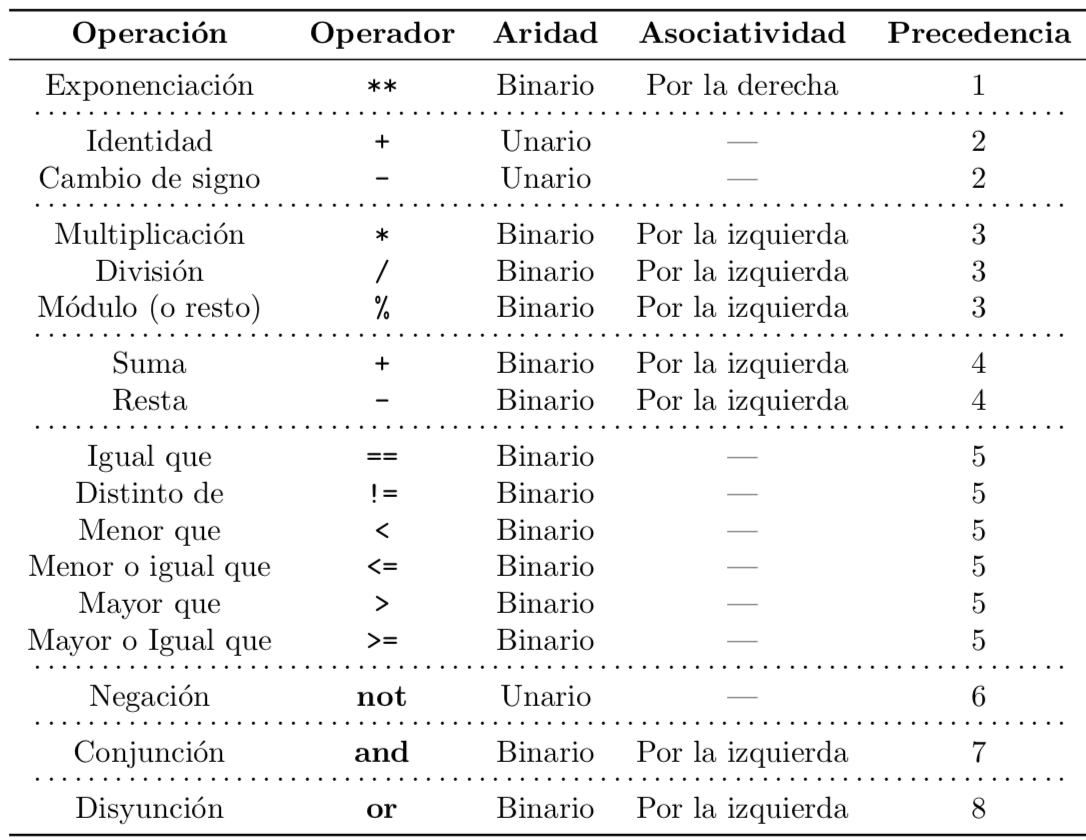
\includegraphics[width=.8\textwidth]{input/01-PythonLenguaje-fig/prioridadOperadores}}}

\caption{Orden de Precedencia \footnotesize Fuente: \texttt{Introducción a la Programación con Python} (página 37)}
\label{fig:precedencia}

\end{figure}


\paragraph{Mutabilidad y Casting.}

Una variables es \key{mutable} si se puede cambiar el valor de la variables sin cambiar su referencia en memoria.

La instrucción \pyv{id(var)} muestra la referencia de la variable {\tt var}.
Esta instrucción nos permite comprobar la mutabilidad de una variable.
Si se hacen dos asignaciones a una variable e \pyv{id()} cambia, la variables es inmutable.
Números, booleanos y strings son inmutables.  \hfill Compruébalo !!

	
	
El \key{casting} es el proceso por el que el valor de una variable se interpreta como otro tipo de dato.
Python no admite casting, pero sí tiene funciones para el \key{cambio de tipo}: 
	\pyv{int()}, \pyv{float()}, \pyv{str()}.




%%%%%%%%%%%%%%%%%%%%%%%%%%%%%%%%%%
%%%%%%%%%%%%%%%%%%%%%%%%%%%%%%%%%%

%%%%%%%%%%%%%%%%%%%%%%%%%%%%%%%%%%
%%%%%%%%%%%%%%%%%%%%%%%%%%%%%%%%%%
% --------------------------------------------------------
\label{subsec:ProgramacionEstructurada}

\subsection*{2.E.4 Programación Estructurada}
\addcontentsline{toc}{subsection}{2.E.4 Programación Estructurada}


La programación estructurada es un paradigma de programación que se basa en el \concepto{Teorema del Programa Estructurado}, propuesto por Böhm-Jacopini,  que demuestra que todo programa puede escribirse utilizando tres estructuras básicas, llamadas \key[red]{estructuras de control}:
\begin{itemize}
\item \key{Estructura secuencia}, consta de una secuencia de instrucciones directas.
\item \key{Estructura condicional}, que consta de una sentencias condicional y sus correspondiente cuerpos.
\item \key{Estructura iterativa}, que consta de bucles (o sentencias iterativas).
\end{itemize}


%--------------------------------------------------------------------------------
\paragraph{Estructura Secuencial.}

Consta de una secuencia de \key{órdenes directas}.
El conjunto de instrucciones \textbf{vienen dadas por el lenguaje} de programación.

\begin{itemize}
\item \key{Sentencias de Asignación}, consistentes en el paso de valores de una expresión o literal a una zona de la memoria.

\item \key{Lectura}, \pyv{input()}, consistente en recibir desde un dispositivo de entrada algún dato.

\item \key{Escritura}, \pyv{print()}, consiste en mandar a un dispositivo de salida algún valor.

\item \key{Tamaño}, \pyv{len()}, calcula el número de datos que tiene una secuencia (p.e. un string).

\item \key{Identificación}, \pyv{id()}, retorna la referencia de una variable.

\item \key{Tipo}, \pyv{type()}, indica el tipo de dato de un literal o de una variable.

\item ...
\end{itemize}

En \key[red]{Python} tenemos: 
	\begin{itemize}
	\item \textbf{Sentencias de asignación:} {\footnotesize \url{https://docs.python.org/3/reference/simple_stmts.html}}
	\item \textbf{Built-in Functions:} \footnotesize \url{https://docs.python.org/3/library/functions.html}
	\end{itemize}



%--------------------------------------------------------------------------------
\paragraph{Estructura condicional.}

Es  aquella que ejecuta ciertas órdenes si se cumple una condición booleana.

En \key[red]{Python} se usa la sentencia compuesta con cláusulas \cm{if}, \cm{elif}, \cm{else}.

\begin{itemize}
\item Condicional simple. 


\hfil
\begin{minipage}{.3\textwidth}
\begin{pyverbatim}[][frame=single, fontsize=\footnotesize]
if condicion:
    estructura
\end{pyverbatim}
\end{minipage} 
\begin{minipage}{.3\textwidth}
\begin{pyverbatim}[][frame=single, fontsize=\footnotesize]
if condicion: sentencia  # Inline
\end{pyverbatim}
\end{minipage}


\item Condicional doble. 


\hfil
\begin{minipage}{.3\textwidth}
\begin{pyverbatim}[][frame=single, fontsize=\footnotesize]
if condicion:
    estructura_if
else:
    estructura_else
\end{pyverbatim}
\end{minipage}
\begin{minipage}{.5\textwidth}
\begin{pyverbatim}[][frame=single, fontsize=\scriptsize]
var = exp_si_true  if  condicion else exp_si_false # Inline
\end{pyverbatim}
\end{minipage}



\item Condicional anidado.

\hfil
\begin{minipage}{.5\textwidth}
\begin{pyverbatim}[][frame=single, fontsize=\footnotesize]
if condicion1 [op condicion2 [op condicion3] ... ]:
    estructura_if
elif condicion:
    estructura_else_if
else  # Casi obligado si se usa elif.
    estructura_else
\end{pyverbatim}
\end{minipage}

\end{itemize}




%--------------------------------------------------------------------------------
\paragraph{Estructura Iterativa.}
%\small 


La versión imperativa de esta estructura consta de los siguientes pasos:

\begin{enumerate}\setlength{\itemsep}{0mm} \small
\item Se parte de una variable, que se llamará \key{variable de control} y que se inicializará a cierto valor. 

\item Entonces se comprueba una \key{condición} booleana donde interviene la variable de control. 

\item Si la condición es cierta, entonces se ejecutarán nuevas \key{estructuras}. 

\item Entres las \key{estructuras} habrá alguna secuencial que \key[magenta]{modifique la variable de control}.

\item Se vuelve paso 2.
\end{enumerate}

El proceso \key{se repite} hasta que la variable de control tome un valor que hace que la condición booleana es falsa.

En \cm[red]{Python} se usa la sentencia \cm{while}:

\begin{pyverbatim}[][frame=single, fontsize=\footnotesize]
control = valor_inicial
while expresion_booleana_con_la_var_de_control:
    estructuras
    modificar la variable de control
else: # opcional
   estructuras
\end{pyverbatim}


El bloque \cm{else} \key{no se realizará} si se ejecutara la sentencia \cm{break} en el bloque \cm{while}.


Existen dos sentencias, \cm{break} y \cm{continue}, que te pueden ser útiles:
%\small 

\begin{itemize}

\item \cm{break} 

\begin{itemize}
\item Solo puede ocurrir sintácticamente en un bucle \cm{for}\footnote{El bucle \cm{for} se estudiará en POO.} o \cm{while}.
\item Terminará el bucle adjunto más cercano y omitirá la cláusula opcional \cm{else}.
\end{itemize}

\item \cm{continue} 

\begin{itemize}
\item Solo puede ocurrir sintácticamente en un bucle \cm{for} o \cm{while}.
\item Continúa con la siguiente iteración del bucle  más cercano.
\item No ejecutará lo que aparezca después de \cm{continue} 
\end{itemize}

\end{itemize}


\begin{ejercicio}
Aquí hay un error muy común ?`cuál?

\hfil\begin{minipage}{.8\textwidth}
\begin{pyverbatim}[][frame=single]
control = 1
while control < 10:   # Se puede cambiar la condición
    if control % 2 == 0:
        continue
    elif control % 5 == 0:
        break
    print(control, end=" ")
    control = control + 1  # Se debe modificar la var. de control
else:
    print("No debería ejecutarse")
\end{pyverbatim}
\end{minipage}
\end{ejercicio}






%%%%%%%%%%%%%%%%%%%%%%%%%%%%%%%%%%
%%%%%%%%%%%%%%%%%%%%%%%%%%%%%%%%%%
% --------------------------------------------------------
\label{subsec:ProgramacionProcedimental}
\subsection*{2.E.5 Programación Procedimental}
\addcontentsline{toc}{subsection}{2.E.5 Programación Procedimental}

Una \key{función} es una \textbf{secuencia} de instrucciones identificada con un \textbf{nombre} que retorna un valor.  En \cm[red]{Python} una función puede retornar varios valores y, en este caso,
 \key{``empaqueta''} todos los datos de retorno en un tipo de datos llamado \key{tupla}. 


\hfil
\begin{minipage}{.65\textwidth}
{\footnotesize
\begin{pyverbatim}[][frame=single]
def nombre_funcion ( lista de parámetros ) -> tipo de dato de retorno:  
   estructuras de la función
   return valores 
\end{pyverbatim}
}
\end{minipage}



Un \key{procedimiento} es una función que no tiene la instrucción de retorno.

\hfil
\begin{minipage}{.65\textwidth}
{\footnotesize
\begin{pyverbatim}[][frame=single]
def nombre_procedimiento ( lista de parámetros ) [-> None]:  
   estructuras del procedimiento
\end{pyverbatim}
}
\end{minipage}


Si una función/método tiene $n$-parámetros podemos invocar a la función con $n$-argumentos de tal forma que el $1^{er}$ argumento se sustituya por el $1^{er}$ parámetro, el $2^{o}$ argumento por el $2^{o}$ parámetros, etc ... Son parámetros \key{posicionales}.


\begin{pyverbatim}[][frame=single]
def fun(a, b, c, d):  # Tiene 4 parámetros
    print(a, b, c, d)

fun(1, 2, 3, 4) # Invocamos con 4 parámetros posicionales.
\end{pyverbatim}


Los \key{k-últimos parámetros} de un función pueden ser \key{opcionales}.
	\begin{itemize}
	\item Los opcionales determinan un valor  \key[magenta]{literal} \key{ por defecto}. 
	\item \textbf{Primero} los obligatorios \textbf{y después} los opcionales (o por defecto).
	\end{itemize}

\begin{pyverbatim}[][frame=single]
def fun(a, b, c=3, d=4): #  2 posicionales + 2 opcionales.
    pass
\end{pyverbatim}


 \cm[red]{Python} permite invocar por \key{palabras claves} (keywords).
	\begin{itemize}
	\item Usar \textbf{keyword =}  especifica el nombre del parámetro en la invocación.
	\item El orden de los parámetros pueden cambiarse.
	\item En la declaración de la función, los keywords siempre se pondrán al final.
	\end{itemize}

\begin{pyverbatim}[][frame=single]
# Para la función anterior
fun(b=2, d=4, a=1, c=3) # Invocamos con 4 keywords.
fun(1, 2, d=4, c=3) # Los keywords al final
fun(d=4, 1, 2, c=3) # Incorrecto
\end{pyverbatim}



Cuando no se conoce el número de argumentos que se usarán, se usa el  \key{Packing Arguments} (empaquetamiento de argumentos) con el operador \key{*}.


\begin{pyconsole}[][frame=single]
def fun(*args):   # Empaquetará todos los argumentos
    print(args)

fun(1, 2, 3, 4)   # Invocación desempaquetada
\end{pyconsole}

En el ejemplo, todos los argumentos se agrupan en una \key{tupla}.

También existe el \key{Unpacking Arguments.} Dada una función/método con varios parámetros podemos empaquetar los argumentos con \key{*}.

\hfil
\begin{pyconsole}[][frame=single]
def fun(a, b, c, d):   # Desempaquetará si le envían \
    print(a, b, c, d)  # los argumentos empaquetados

lista = [1, 2, 3, 4] # Las listas las veremos más tarde.
fun(*lista)          # Invocación empaquetada
\end{pyconsole}



Para acceder a uno de lo argumentos empaquetados se usan \key{índices}:

\begin{pyconsole}[][frame=single, fontsize=\footnotesize]
def fun(*args): 
    print(len(args), args[1]) # Muestra el cardinal y el 2o argumento

fun(1, 2, 3, 4)
\end{pyconsole}


Estaría mejor acceder a ellos con un nombre (keyword). De hecho,
podemos \key{empaquetar y usar keywords} usando \textbf{diccionarios}, con \cm{**}. \textbf{Un diccionario es} como un array pero los índices se sustituyen por claves.

\begin{pyconsole}[][frame=single, fontsize=\footnotesize]
def fun(**kwargs): 
    print(f"{len(kwargs)} elementos", kwargs) # Muestra el diccionario

fun(a=1, b=2, c=3, d=4)    # Invocación con keywords
diccionario = {'p1': 1, 'p2': 2, 'p3':3}  # Los veremos
fun(**diccionario)         # Invocación con empaquetado
\end{pyconsole}




\noindent Si se quieren usar los 3 modos de pasar argumentos, el orden debe ser:
\begin{enumerate}
\item posicionales 
\item empaquetados sin keyword
\item empaquetados con keyword
\end{enumerate} 



\begin{pyconsole}[][frame=single, fontsize=\footnotesize]
def fun(a, b, *args, **kwargs): 
    print(a, b)  # Muestra los posicionales
    print(args)  # Muestra los empaquetados sin keyword
    print(kwargs)# Muestra los empaquetados con keyword

fun(1, 2, 3, 4, 5, p1=6, p2=7, p3=8)
\end{pyconsole}

\begin{ejercicio}
Se define \pyv{def func(x, y, op = "+")}. ?`Cuánto valdrá \cm{x}, \cm{y} y \cm{op} en los siguientes casos?

\begin{itemize*}
\item \pyv{func(2, 3, "*") }
\item \pyv{func( (2, 3), "*") }
\item \pyv{func( *(2, 3), "*")} \\
\item \pyv{func( *(2, 3, "*"))}
\item \pyv{func( (2, 3, "*"), 4)}
\item \pyv{func( *(2, 3, "*"), 4)}
\end{itemize*}
\end{ejercicio}



%--------------------------------------------------------------------------------
\paragraph{Docstrings.}

Toda función debe contener su \key{especificación informal}.
La documentación se hace en Python mediante \key{docstrings}: Cadenas que empiezan y terminan con triple comillas (simples o dobles)
Existen varios \key{formatos} (lenguajes de marcas):
\begin{itemize}
\item reStructuredText. El estandar de Python.
\item Google. La mejor alternativa "no-nativa".
\item Numpy. La propuesta de Numpy.
\item etc ...
\end{itemize}


\hfil\begin{minipage}{.4\textwidth}
\begin{pyverbatim}[][frame=single, fontsize=\footnotesize]
def func (x: int) -> str:
    """
    Función general que no hace nada
    reStructuredText
    
    :param x: La entrada, es entero
    :return: El valor de retorno
    """
    pass
\end{pyverbatim}
\end{minipage}
\begin{minipage}{.4\textwidth}
\begin{pyverbatim}[][frame=single, fontsize=\footnotesize]
def func (x: int) -> str:
    """
    Función general que no hace nada
    Google
    
    Args:
        x: La entrada, es entero

    Returns:
        El valor de retorno
    """
    pass
\end{pyverbatim}
\end{minipage}






%%%%%%%%%%%%%%%%%%%%%%%%%%%%%%s%%%%
%%%%%%%%%%%%%%%%%%%%%%%%%%%%%%%%%%
\paragraph{Funciones Lambda o Anónimas.}

El $\lambda$-cálculo es un sistema formal matemático desarrollado en los años 1930s diseñado para trabajar con la noción de  función, aplicación de funciones y  recursión. Proporciona una semántica simple para la computación y la primera simplificación es que el $\lambda$-cálculo \textbf{trata las funciones de forma anónima}.
La escritura anónima de $\color{red}{\displaystyle \operatorname {square\_sum} (x,y)=x^{2}+y^{2}}$ es  $\color{blue}{\displaystyle (x,y)\mapsto x^{2}+y^{2}}$.


En \key[red]{Python} las expresiones anónimas se llaman \key{Funciones Lambda} y
tiene la siguiente expresión: 

\centerline{\fbox{\pyv{lambda argumentos: expresión}}}

En la definición deberá tener en cuenta:
	\begin{itemize}
	\item Puede usar cualquier número de argumentos.
	\item Solo habrá una única expresión.
	\end{itemize}
	

\hfil\begin{minipage}{.4\textwidth}
\begin{pyconsole}[][frame=single, fontsize=\footnotesize]
el_doble = lambda x: x * 2
print(el_doble(10))
suma = lambda x, y: x + y
print(suma(4, 5))
acotado = lambda x: 4 <= x <= 8
print(acotado(5))
\end{pyconsole}
\end{minipage}


Son útiles junto con funciones clausura como \pyv{map()}, \pyv{filter()}, \cm{reduce}(), ... para trabajar con colecciones.  Se verán más adelante.






%%%%%%%%%%%%%%%%%%%%%%%%%%%%%%%%%%
%%%%%%%%%%%%%%%%%%%%%%%%%%%%%%%%%%

%--------------------------------------------------------------------------------
\subsection*{2.E.6 Programación Modular}
\addcontentsline{toc}{subsection}{2.E.6 Programación Modular}



Es un paradigma de programación que consiste en \key{dividir un gran programa} (posiblemente de  miles de líneas) \key{en módulos} (ficheros). 
Los módulos constan a su vez de \key{funciones}, \key{variables}, \key{clases}. 
Algunos módulos usarán otros módulos pero habrá uno (y solo uno), llamado \key{módulo principal}, que no puede ser usado por los demás módulos.
El módulo principal es el encargado de ir resolviendo cada una de las subtareas.


En \cm[red]{Python} la modularidad se consigue con \cm{import}. Ejemplo de uso de módulos:

\begin{minipage}{.31\textwidth}  
\begin{pyconsole}[][frame=single]
import math 
print("PI=", math.pi)
\end{pyconsole}
\end{minipage}
%
\begin{minipage}{.31\textwidth}
\begin{pyconsole}[][frame=single]
import math as m
print("PI=", m.pi)
\end{pyconsole}
\end{minipage}
%
\begin{minipage}{.33\textwidth}
\begin{pyconsole}[][frame=single]
from math import pi, cos
print("cos(PI)=", cos(pi))
\end{pyconsole}
\end{minipage}




%%%%%%%%%%%%%%%%%%%%%%%%%%%%%%%%%%
%%%%%%%%%%%%%%%%%%%%%%%%%%%%%%%%%%

%--------------------------------------------------------------------------------
\label{subsec:ClasesEnPython}
\subsection*{2.E.7 Programación Orientada a Objetos \label{subsec:POO}}
\addcontentsline{toc}{subsection}{2.E.7 Programación Orientada a Objetos}


La estructura básica para definir una clase en \cm[red]{Python} es la siguiente:

\hfil \begin{minipage}{.75\textwidth}
\begin{pyverbatim}[][frame=single]
class NombreDeLaClase: # Notación Camel
    def __init__(self, p1, p2, ...):
        self._var1 = p1
        self._var2 = p2
        ...  # más atributos
        
    def metodo1 (self, parametros):
        acciones
            
    def metodo2 (self, parametros):
        acciones
            
     .... # más métodos
        
objeto = NombreDeLaClase(argumentos para __init__)
\end{pyverbatim}
\end{minipage}

\

Todos los métodos que tienen la forma: \cm[blue]{\_\_metodo\_\_}{\tt (...)} se denominan    \key{métodos mágicos}. Destacamos:

\begin{itemize}

\item \pyv{__new__(cls, ...)}. Es el método creador.  \textbf{No debe escribirse nunca}.

\item \pyv{__init__(self, ...)}.   \textbf{Es un método inicializador} de instancia que se invoca siempre, una vez construido el objeto con \pyv{__new__(cls, ...)}.

\item etc ...
\end{itemize}


Trabajar con \key{TDAs} como modelos \key{ayuda} muchísimo  a la resolución de problemas y  diseño de algoritmos; pero al final hay que implementarlos en un lenguaje de programación usando sus \key{tipos de datos integrados}.  Todos los tipos de datos integrados en Python son objetos y, por tanto, si queremos construir nuevos tipos de datos debemos saber cómo construir y manipular nuevos objetos.

Deberá tener presente que Python es un lenguaje de POO puro. En consecuencia, cualquier operación que realice conlleva manipular los atributos del objeto y, por tanto, invocará de forma directa o indirecta a los métodos del objeto.

Por ejemplo, en \underline{todos} los \textbf{Tipos de Datos Numéricos} tenemos estos miembros/métodos y operaciones:
	\begin{itemize}
	\item Miembros: \cm[blue]{.real}, \cm[blue]{.imag}
	\item Métodos: \cm[blue]{.conjugate()}, 
	\item Operaciones: \cm{+}, \cm{-}, \cm{*}, \cm{/}, \cm{//}.
	\item Los métodos mágicos sobre operaciones matemáticas, asignaciones extendidas, operaciones unarias y operaciones de comparación.
	\end{itemize}

Esto quiere decir que cuando realice una operación numérica  invocará al método mágico correspondiente. Por ejemplo,  
	\begin{itemize}
	\item Cuando escriba \key{3+5}, internamente se ejecutará \pyv{3.__add__(5}). Siendo el \key{3} y el \key{5} dos objetos.
	\item Si escribe \key{3-5}, internamente se ejecutará \pyv{3.__sub__(5)}.
	\item etc ...
	\end{itemize}

Lo mismo ocurre cuando invoque a un función sobre un número. Por ejemplo, invocando a \key{abs(3}) estará invocando a \pyv{3.__abs__()}.  También ocurre lo mismo al usar operadores de comparación: usar \cm{<} es invocar al método \pyv{.__lt__()}, usar \cm{==} invocará al método \pyv{.__eq__()}, etc ...

De entre todos los operadores el más esencial es sin duda la asignación \cm{=}. Cada vez que realice una asignación de la forma estará construyendo un objeto nuevo y cada vez que se crea un objeto nuevo se invocará al método \pyv{.__init__()}. Esto es muy importante a tener en cuenta porque:

\begin{itemize}
\item A ser un lenguaje no tipado, la asignación determina su tipo. En consecuencia una variable puede referenciar incialmente a un entero para terminar referenciando a una lista.

\begin{pyverbatim}[][frame=single]
a = 2  % a es un objeto entero
a = 2 == 3  % a es un objeto booleano
a = NombreDeLaClase(p1, p2) % a es un objeto de NombreDeLaClase
\end{pyverbatim}

 
 
\item Todas las variables tienen un ámbito local salvo que  se diga lo contrario (se explicará  posteriormente).
\end{itemize}

\noindent Para completar los \textbf{Tipos de Datos Numéricos} en  Python, indicar que se tienen los siguientes.

\begin{itemize}	
\item \textbf{Enteros:}
	\begin{itemize}
	\item Una variable se declara entera si se le asigna un número sin punto decimal.
	\item Función constructora: \cm{int()}. 
	\item Métodos: \cm[blue]{.bit\_length()}: N$^o$ de bits necesarios.
	\item Funciones: \key{bin}(n). Convierte a binario.
	\end{itemize}
	
\item \textbf{Reales:}
	\begin{itemize}
	\item Una variable se declara real si se le asigna un número con punto decimal.
	\item Función constructora: \cm{float()}. 
	\item Métodos: \cm[blue]{.is\_integer()}: True si el valor es igual al de su parte entera.
	\end{itemize}
	
\item \textbf{Complejos:}
	\begin{itemize}
	\item Constructor: \cm{complex([real[, imag]])}
	\end{itemize}
\end{itemize}

Podemos aumentar el conjunto de datos numéricos usando librerías.
Destacamos aquí el módulo \textbf{Fracciones:}
	\begin{itemize}
	\item Requiere \cm{from fractions import Fraction}
	\item Constructores: \cm{Fraction(numerator=0, denominator=1)}, \cm{Fraction(float)}, \cm{Fraction(string)}, ...
	\item Miembros: \cm[blue]{.numerator}, \cm[blue]{.denominator}
	\item Métodos: \cm[blue]{.as\_integer\_ratio()}: simplifica la fracción.
	\item \url{https://docs.python.org/3/library/fractions.html}
	\end{itemize}	
	
\


Otros tipos de datos integrados son los \textbf{Tipos de Datos Booleanos.}
Usa las constantes True y False. Una variable a la que se le asigne uno de estos valores será una variable booleana.  Las expresiones booleanas se construyen con:
	\begin{itemize}
	\item Comparaciones: \cm{x == y}, \cm{x != y}, \cm{x > y}, \cm{x >= y}, \cm{x <\ y}, \cm{x <= y}
	\item Operaciones: \cm{e1 and e2}, \cm{e1 or e2}, \cm{not e}
	\end{itemize}
	
Recuerde que todas estas operaciones invocará a sus correspondiente método mágicos.
	

Los TDAs más relevantes requieren el uso de colecciones.
\cm[red]{Python} proporciona un conjunto de tipos de datos llamados \textbf{secuencias} (colecciones) o tipos de datos secuenciales. Se explicarán con más detenimiento en sesiones posteriores (de teoría/prácticas).



\paragraph{Recuerde seguir  PEP 8 para las normas de estilo.}
\paragraph{PEP 8 -- Style Guide for Python Code: \url{https://www.python.org/dev/peps/pep-0008/}
}	











\


\

\

\centerline{\Large \bf Ejercicios}

\

\formatoEjercicio



%%%%%%%%%%%%%%%%%%%%%%%%%%%%%%%%%%%%%%%%%%%%%%%%%% 
\separacion
\section{Un clase para números positivos} \label{sec:numerosPositivos}
\objetivo{1}{B}{\cm{assert}, \cm{isinstance} y algún método mágico}

Con la clase \cm[black]{Positivo} se quiere implementar los números
naturales (enteros positivos). 
Para su implementación, sabemos que no existe este tipo de dato pero sí un tipo de dato para los naturales (\cm{int}). Por ello, se opta por esta implementación:

\begin{pyverbatim}[][frame=single]
class Positivo:
    __slots__ = '_num'

    def __init__(self, num: int):
        pass

    def __str__(self) -> str:
        pass

def una_prueba():
    pass
          
if __name__ == '__main__':
    una_prueba()
\end{pyverbatim}

Debes completar el código teniendo en cuenta los siguientes puntos, consultando la documentación de \cm[red]{Python} si fuera necesario:

\begin{itemize}
\item El atributo \cm{\_num} es el que almacenará el número entero positivo. De acuerdo a esto ?cuál es la función de abstracción? 

\item El método de inicialización \cm{\_\_init\_\_()} debe generar un error si se intenta crear un objeto con un entero no positivo. Usa las instrucciones \cm{assert} y \cm{isinstance} para generar un error si el valor dado no es un entero positivo.  De acuerdo a esto ?`cuál es el invariante de la representación?

\item El método \cm{\_\_str\_\_() : str} retornará en forma de string (\cm{str}) el valor de \cm{\_num}.
\end{itemize}



%\begin{pycode}
%class Positivo:
%    def __init__(self, num):
%        assert num>0, "Error, el número dado no es positivo"
%        assert isinstance(num, int), "Error, el número no es un entero"
%        self._num = num
%    def __str__(self):
%        return str(self._num)
%
%el_tres = Positivo(3)    # Crea un objeto que representa al 3
%print(el_tres)           # Muestra 3
%el_cero = Positivo(0)    # Debe mostrar un error
%el_pi = Positivo(3.14)   # Debe mostrar un error
%
%\end{pycode}


Como ejemplo de uso define la función \pyv{def una_prueba()} con el siguiente código.

\begin{pyverbatim}[][frame=single]
el_tres = Positivo(3)    # Crea un objeto que representa al 3
print(el_tres)           # Muestra 3
el_cero = Positivo(0)    # Debe mostrar un error
el_pi = Positivo(3.14)   # Debe mostrar un error
\end{pyverbatim}



% - - - - - - - - - - - - - - - - - - - - - - - - - - - - - - - - - - - - - - - - - - - -



%\input ejercicios/05-Funciones/FuncionesSencillasSol.tex


 
%%%%%%%%%%%%%%%%%%%%%%%%%%%%%%%%%%%%%%%%%%%%%%%%%% 
\separacion
\section{TDA Fecha Simple} \label{sed:TDAFechaSimple}
\objetivo{1}{B}{Implementación de Fecha con clases}
%Data Structures and Algorithms Using Python.pdf, pág 15}

Implementa el TDA fecha usando la representación indicada en el Ejemplo \ref{ejem:FechaSimple}. Para ello debes completar el siguiente código:

\begin{pyverbatim}[][frame=single, fontsize=\small]
class Fecha:
    __slots__ = '_dia', '_mes', '_agno'

    def __init__(self, dia: int, mes: int, agno: int):
        pass

    def _set_agno(self, agno: int) -> None:
        pass

    def _set_mes(self, mes: int) -> None:
        pass

    def _set_dia(self, dia: int, mes: int) -> None:
        pass

    def get_dia(self) -> int:
        pass

    def get_mes(self) -> int:
        pass

    def get_agno(self) -> int:
        pass

    def __str__(self) -> str:
        pass
\end{pyverbatim}


Ten en cuenta que:
\begin{itemize}
\item El método \pyv{def __init__()} debe invocar a los métodos \pyv{def _set_xxx}. Por ejemplo, se invocará a la asignación del año como \pyv{self._set_agno(agno)}.

\item Los métodos \pyv{def _set_xxx} controlarán si los argumentos son correctos, en especial para los días (que dependen de los meses).
Usa las instrucciones \cm{assert} y \cm{isinstance} para generar un error si los valores dados no se corresponden con la especificación. 
No es necesario comprobar que los años sean bisiestos.

Observa que empiezan con ``guión bajo''. Esto quiere decir que los métodos \cm{\_set\_xxx} no deberían ser invocados desde otras clases (es decir, no se puede modificar una fecha una vez creada). 

\item Los métodos \pyv{def get_xxx} permiten consultar los datos de un fecha.
Estos métodos no empiezan con ``guión bajo''. Esto quiere decir que pueden ser invocados desde otras clases. 

\item El método \pyv{def __str__()} retornará la cadena ``dd/mm/aa''.
Se invocará cuando uses la instrucción \pyv{print()}.

\item Construye un método de prueba para imprimir fechas válidas y crear fechas inválidas (contemplando todas las posibilidades del invariante de la representación.
\end{itemize}


% - - - - - - - - - - - - - - - - - - - - - - - - - - - - - - - - - - - - - - - - - - - -



 
%%%%%%%%%%%%%%%%%%%%%%%%%%%%%%%%%%%%%%%%%%%%%%%%%% 
\separacion
\section{TDA Fecha Simple con Positivo} \label{sec:FechaSimplePositivos}
\objetivo{1}{B}{Otra Implementación de Fecha}
%Data Structures and Algorithms Using Python.pdf, pág 15}

Implementa el TDA Fecha del ejercicio anterior cambiando el tipo \cm{int} del día y del mes por el tipo \cm{Positivo} del primer ejercicio.

Crea un fichero .py con un nombre nuevo y reescribe \pyv{class Fecha}. No le cambies el nombre a la clase, solo al fichero.


% - - - - - - - - - - - - - - - - - - - - - - - - - - - - - - - - - - - - - - - - - - - -



% - - - - - - - - - - - - - - - - - - - - - - - - - - - - - - - - - - - - - - - - - - - -



%\input ejercicios/05-Funciones/FuncionesSencillasSol.tex



%%%%%%%%%%%%%%%%%%%%%%%%%%%%%%%%%%%%%%%%%%%%%%%%%% 
\separacion
\section{Un clase para cilindros} \label{sec:TDACilindro}
\objetivo{1}{B}{función de abstracción, invariante de la representación}

Se quiere construir el TDA Cilindro Recto con las operaciones básicas del cálculo de volumen y superficie.
\begin{itemize}
\item Defina el TDA.
\item Defina la función de abstracción.
\item Defina el invariante de la representación.
\item Implemente en Python el TDA.
\item Añada a la implementación el método mágico \pyv{__str__()} para imprimir toda la información disponible de un cilindro.
\end{itemize}


 
%%%%%%%%%%%%%%%%%%%%%%%%%%%%%%%%%%%%%%%%%%%%%%%%%% 
\separacion
\section{TDA Fracción} \label{sec:TDAFraccion}
\objetivo{2}{B}{Implementación de Fracción}

Escribe al definición informal del TDA, su función de abstracción y el invariante de la representación.

Responde a lo indicado e implementa el TDA teniendo en cuenta que una fracción \cm{fr} puede usar los siguientes métodos: 
\begin{itemize}
\item \cm{fr.suma(f: Fraccion)} realiza la asignación: \cm{fr = fr+f}. 
\item \cm{fr.resta(f: Fraccion)} realiza la asignación: \cm{fr = fr-f}. 
\item \cm{fr.multiplica(f: Fraccion)} realiza la asignación: \cm{fr = fr * f}. 
\item \cm{fr.divide(f: Fraccion)} realiza la asignación: \cm{fr = fr / f}.
\item \cm{fr.simplifica()} para obtener su fracción más simplificada posible.
\end{itemize}

¿Cuáles son los métodos mágicos que debes de implementar para realizar estas operaciones \cm{f1==f2} y \cm{f1<f2}?

Te puede interesar el algoritmo de Euclides \url{https://es.wikipedia.org/wiki/Algoritmo_de_Euclides#Descripci%C3%B3n_formal}




% - - - - - - - - - - - - - - - - - - - - - - - - - - - - - - - - - - - - - - - - - - - -

 
%%%%%%%%%%%%%%%%%%%%%%%%%%%%%%%%%%%%%%%%%%%%%%%%%% 
\separacion
\section{Adivina el número}
\objetivo{1}{-}{Lenguaje Imperativo en Python}



Construir el siguiente juego de adivinación de números. 


\begin{itemize}% [leftmargin=-.1in, rightmargin=-.3in]\setlength{\itemsep}{3mm}
\item El humano  introduce un número.
\item El ordenador debe de adivinar el número introducido por el usuario.
\item El humano indicará si el número dado por el ordenador es mayor o menor al que ha introducido.
\item La partida no termina hasta que el ordenador lo adivine.
\item Los números estarán en el intervalo $[0, 100]$.
\item Cuando lo adivine se mostrará un mensaje indicando el número de intentos realizados.
\item Descubierto el número, se preguntará si se quiere  otra partida.
\item Si no se quiere  otra partida se preguntará si se desea salir del juego.
\item Si se deseara salir, se debe confirmar la respuesta. Si la respuesta es ``no confirmo'', volverá a preguntar si quiere otra partida.
\item Realizar un programa que haga todo  lo anterior sin la participación de humano alguno. Por comodidad se puede suponer siempre que el número dado por el humano es siempre el mismo.
\end{itemize}

Resuelve este ejercicio usando solo programación estructurada (sin clases). 
\textbf{Si tienes problemas para resolver este ejercicio, probablemente te falte base para poder afrontar la POO.}





